\fancyhead[C]{\normalsize\textbf{$\qquad$ Teil II: Multiple-Choice}}
\section*{Aufgabe 2 (32 Punkte)}
\vspace{0.4cm}
\subsection*{\frage{1}{4}}
Die Funktion $ f(x,y) \ = \ (x-2)^2 -y^2 $ hat einen Sattelpunkt beim Punkt $ P \ = \ (2,0) $. Welche der folgenden Aussagen ist korrekt?
\renewcommand{\labelenumi}{(\alph{enumi})}
\begin{enumerate}
	\item Die Funktion $ f $ hat unter der Nebenbedingung $ 2x \ - y \ - \ 4 \ = \ 0 $ ein lokales Minimum beim Punkt $ P $.
	\item Die Funktion $ f $ hat unter der Nebenbedingung $ 2x \ - y \ - \ 4 \ = \ 0 $ einen Sattelpunkt beim Punkt $ P $.
	\item Die Funktion $ f $ hat unter der Nebenbedingung $ -x \ - 2y \ - \ 4 \ = \ 0 $ einen Sattelpunkt beim Punkt $ P $.
	\item Die Funktion $ f $ hat unter der Nebenbedingung $ -\frac{1}{2}x \ - y \ + \ 1 \ = \ 0 $ ein lokales Minimum beim Punkt $ P $.
	\item Die Funktion $ f $ hat unter der Nebenbedingung $ -\frac{1}{2}x \ - y \ + \ 1 \ = \ 0 $ ein lokales Maximum beim Punkt $ P $.
\end{enumerate}
\ \\
\textbf{Lösung:}
\begin{mdframed}
\underline{\textbf{Vorgehensweise:}}
\renewcommand{\labelenumi}{\theenumi.}
\begin{enumerate}
\item Prüfe, ob $ P $ die Nebenbedingung erfüllt.
\item Verwende Substitution für die übrigen Antwortmöglichkeiten.
\end{enumerate}
\end{mdframed}

\underline{1. Prüfe, ob $ P $ die Nebenbedingung erfüllt}\\
Die Antwortmöglichkeiten (a),(b) und (d),(e) besitzen jeweils identische Nebenbedingungen.
Durch Einsetzen von $ P $ erhalten wir:
\begin{align*}
	2 x - y -4 = 0 \ &\Rightarrow 2 \cdot 2 -4  = 0 \ \text{NB (a),(b)}\\
	-x  - 2y - 4 = 0 \ &\Rightarrow \ -2 -4 \neq 0 \ \text{NB (c)}\\
	-\frac{1}{2}x - y + 1 = 0 \ &\Rightarrow 2 \cdot 2 -4  = 0 \ \text{NB (d),(e)}
\end{align*}
Von (c) wird die Nebenbedingung nicht erfüllt, die übrigen Antwortmöglichkeiten müssen wir untersuchen.\\
\\
\underline{2. Verwende Substitution für die übrigen Antwortmöglichkeiten}\\
Da die Nebenbedingung lineare Funktionen sind können wir diese problemlos substituieren.
Wir beginnen mit $ \varphi_1(x,y) = 2x-y -4 = 0 $. Dies können wir durch
\begin{align*}
	2x -y -4 = 0 \ \Leftrightarrow \ y = 2x - 4
\end{align*}
umformen und erhalten damit die Zielfunktion:
\begin{align*}
	F_1(x) = f(x, 2x -4) = (x-2)^2 - (2x-4)^2
	= (x-2)^2 - 4 (x-2)^2
	= -3 (x-2)^2.
\end{align*}
Damit ergibt sich (mit der Kettenregel)
\begin{align*}
	F_1^\prime(x) &= -3 \cdot 2 (x -2 ) = -6 (x-2) \ \Rightarrow \ F_1^\prime(2) = 0\\
	F_1^{\prime \prime}(x) &= -6 < 0,
\end{align*}
womit $ f $ an $ P $ unter der Nebenbedingung $ \varphi_1 $ ein lokales Maximum besitzt. Die Antwortmöglichkeiten (a) und (b) sind also falsch.\\
\\
Wir wenden uns der Nebenbedingung $ \varphi_2(x,y) = - \frac{1}{2} x -y +1 $ zu. Diese können wir durch 
\begin{align*}
	- \frac{1}{2} x -y  +1 = 0 
	\ \Leftrightarrow \
	y = - \frac{1}{2}x +1
\end{align*}
umformen und erhalten die Zielfunktion
\begin{align*}
	F_2(x) = f\left(x,-\frac{1}{2} x +1\right)
	&=
	(x-2)^2 - \left(-\frac{1}{2} x +1\right)^2
	=
	(x-2)^2- \left(-\frac{1}{2}\right)^2 (x - 2)^2\\
	&=
	(x-2)^2 - \frac{1}{4}(x - 2)^2
	= \frac{3}{4} (x-2)^2.
\end{align*}
Damit ergibt sich (mit der Kettenregel)
\begin{align*}
	F_2^\prime(x) &= \frac{3}{4} \cdot 2 (x -2 ) = \frac{3}{4} (x-2) \ \Rightarrow \ F_1^\prime(2) = 0\\
	F_1^{\prime \prime}(x) &= \frac{3}{4} > 0,
\end{align*}
womit $ f $ an $ P $ unter der Nebenbedingung $ \varphi_2 $ ein lokales Minimum besitzt.\\
\\
Damit ist die Antwort (d) korrekt.\\
\\
Alternativ lässt sich die Aufgabe auch über graphische Veranschaulichung lösen.
Die erste Grafik beinhaltet $ f $ mit der Nebenbedingung $\varphi_1(x,y) = 2x -y -4 = 0$.
\begin{center}
	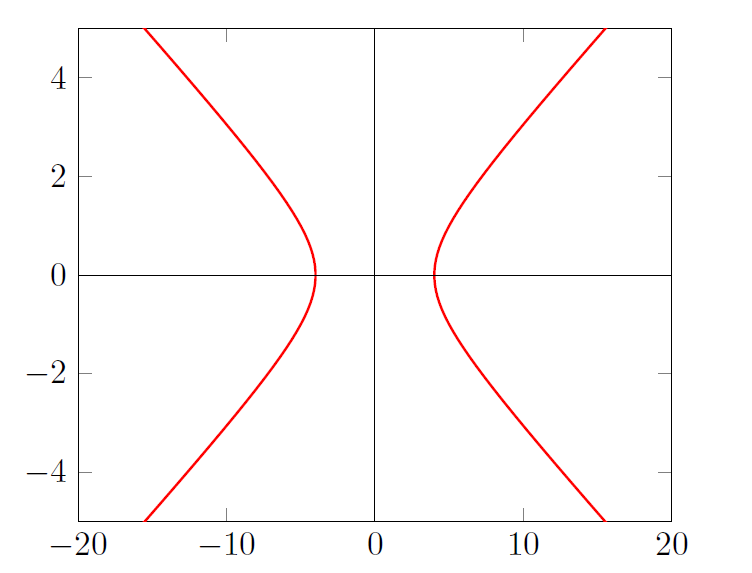
\includegraphics[width=0.6\textwidth]{pictures/aufgabe2_1_1}
\end{center}
Man sieht, dass $ f $ an $ P $ unter $ \varphi_1 $ ein lokales Maximum besitzt, womit die Antwortmöglichkeiten (a) und (b) ausgeschlossen sind.\\
Die zweite Grafik beinhaltet $ f $ mit der Nebenbedingung $\varphi_2(x,y) = -\frac{1}{2}x -y +1 = 0$.
\begin{center}
	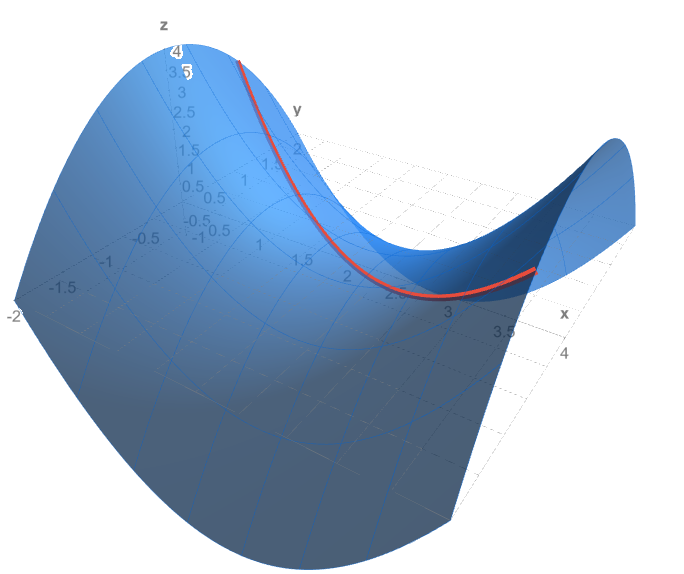
\includegraphics[width=0.6\textwidth]{pictures/aufgabe2_1_2}
\end{center}
Man erkennt, dass $ f $ an $ P $ unter $ \varphi_2 $ ein lokales Minimum besitzt.
\newpage

\subsection*{\frage{2}{3}}
Sei $ f \ : \ D_f \to \mathbb{R} $ eine positive Funktion zweier reeller Variablen, welche ein lokales Maximum beim Punkt $ P = (5,2)  $ hat.
Sei $ h  \ : \ D_f \to \mathbb{R} $ die Funktion definiert durch
\begin{align*}
	h(x,y) = e^{\sqrt{f(x,-y)}}.
\end{align*} 
Welche der folgenden Aussagen ist korrekt?
\renewcommand{\labelenumi}{(\alph{enumi})}
\begin{enumerate}
	\item Die Funktion $ h $ hat ein lokales Maximum beim Punkt $ Q = (-5,2). $
	\item Die Funktion $ h $ hat ein lokales Maximum beim Punkt $ Q = (5,-2). $
	\item Die Funktion $ h $ hat ein lokales Minimum beim Punkt $ Q = (-5,2). $
	\item Die Funktion $ h $ hat ein lokales Minimum beim Punkt $ Q = (5,-2). $
	\item Wir können die Extremstellen von $ h $ nicht analysieren, ohne mehr Informationen zur Funktion $ f $ zu haben.
\end{enumerate}
\ \\
\textbf{Lösung:}
\begin{mdframed}
	\underline{\textbf{Vorgehensweise:}}
	\renewcommand{\labelenumi}{\theenumi.}
	\begin{enumerate}
		\item Verwende die Monotonie.
	\end{enumerate}
\end{mdframed}
\underline{1. Verwende die Monotonie}\\
Da $ f(x,y) $ in  $ (5,2) $ ein lokales Maximum hat, besitzt $ f(x,-y) $ in $ (5,-2) $ ein Maximum. 
Es gilt im Allgemeinen gilt: $ f(x,y) $ hat ein lokales Maximum in $ (x_0,y_0) $ genau dann, wenn $ f(x,-y) $ ein lokales Maximum in $ (x_0,-y_0) $ besitzt.
Weiter erhalten streng monotone Funktionen die lokalen Extrema.
Da die Exponentialfunktion und die Wurzelfunktion streng monoton sind, ist deren Zusammensetzung auch streng monoton. Damit besitzen $ h(x,y) $ und $ f(x,-y) $ dieselben Extrema. Somit ist $ (5,-2) $ ein lokales Maximum von $ h$. 


\newpage
\subsection*{\frage{3}{3}}
Sei $ F $ die Stammfunktion der stetigen Funktion $ f $ einer reellen Variable $ x $ und sei $ g $ eine lineare Funktion, d.h. $ g(x) = ax +b $ für die Parameter $ a,b \in \mathbb{R} $. Das unbestimmte Integral
\begin{align*}
	\int f(x) g(x) \ dx.
\end{align*}
ist gleich:
\renewcommand{\labelenumi}{(\alph{enumi})}
\begin{enumerate}
	\item 
	$ a x F(x) + b F(x) - a \int F(x) dx$.
	\item 
	$ g(x) F(x) - a \int f(x) dx$.
	\item 
	$ \left(\frac{1}{2} a x^2 +b x\right) F(x) - \int a F(x) dx$.
	\item
	$ \left(\frac{1}{2} a x^2 +b x\right) F(x) - \int  F(x) g(x) dx$.
	\item 
	Wir können das Integral nicht transformieren, ohne mehr Informationen zur Funktion $ f $ zu haben.
\end{enumerate}
\ \\
\textbf{Lösung:}
\begin{mdframed}
\underline{\textbf{Vorgehensweise:}}
\renewcommand{\labelenumi}{\theenumi.}
\begin{enumerate}
\item Verwende partielle Integration.
\end{enumerate}
\end{mdframed}

\underline{1. Verwende partielle Integration}\\
Wir definieren durch
\begin{align*}
	u(x)  = F(x)  \ &\Rightarrow \ u^\prime(x) = f(x)\\
	v(x) = g(x)  \ &\Rightarrow \ v^\prime (x) = a	
\end{align*}
Funktionen für die partielle Integration. Damit erhalten wir
\begin{align*}
	\int f(x) g(x) \ dx.
	=
	\int u^\prime(x) v(x) \ dx
	=
	u(x) v(x) - \int u(x) v^\prime(x) \ dx
	=
	F(x)(ax+b) - a \int F(x) \ dx
	=
	axF(x) + b F(x) - a \int F(X) \ dx,
\end{align*}
womit die Antwort (a) korrekt ist.

\newpage

\subsection*{\frage{4}{3}}
Sei $ f $ eine \textit{gerade} Funktion, welche die folgenden (Integral-) Gleichungen erfüllt:
\begin{align*}
	\int_{2}^3 f(x) \ dx = 10, \ \textrm{und} \
	\int_1^3 f(x) \ dx = 15.
\end{align*}
Das bestimmte Integral
\begin{align*}
	\int_{-2}^{-1} (2 - f(x) ) \ dx
\end{align*}  
gleich
\renewcommand{\labelenumi}{(\alph{enumi})}
\begin{enumerate}
	\item 
	$ -1 $.
	\item
	$ -2 $.
	\item
	$ -3 $.
	\item
	$ -4 $.
	\item
	Wir haben nicht genügend Informationen, um diesen Wert auszurechnen.
\end{enumerate}
\ \\
\textbf{Lösung:}
\begin{mdframed}
\underline{\textbf{Vorgehensweise:}}
\renewcommand{\labelenumi}{\theenumi.}
\begin{enumerate}
\item Forme das Integral um und verwende, dass die Funktion gerade ist.
\end{enumerate}
\end{mdframed}

\underline{1. Forme das Integral um und verwende, dass die Funktion gerade ist}\\
Mit der Information, dass $f$ gerade ist und den gegebenen Werten für das Integral gilt:
\begin{align*}
	\int_{-2}^{-1} (2 - f(x) ) \ dx
	&=
	\int_{-2}^{-1} 2  \ dx
	-
	\int_{-2}^{-1} f(x) \ dx
	\underset{f \ \text{gerade}}{=}
	2
	-
	\int_{1}^{2} f(x) \ dx\\
	&=
	2 
	-
	\left(\int_{1}^{3} f(x) \ dx - \int_{2}^{3} f(x) \ dx\right)
	=
	2
	-
	(15 - 10)
	=-3
\end{align*}
Damit ist die Antwort (c) korrekt.

\newpage
\subsection*{\frage{5}{4}}
Gegeben seien die Matrizen $ A_{n \times m} $ und $ B_{m \times n} $ für $ m,n \in \mathbb{N} $.\\
\\
Es folgt:
\renewcommand{\labelenumi}{(\alph{enumi})}
\begin{enumerate}
	\item 
	Die Matrix $ (AB)^\top $ hat die Dimensionen $ n \times m $.
	\item 
	Die Matrix $ (AB)^\top $ ist symmetrisch, falls $ A $ symmetrisch ist.
	\item 
	Die Matrix $ (AB)^\top $ ist invertierbar, falls $ \mathrm{rg}(A) = \mathrm{rg}(B) = n $.
	\item 
	Die Matrix $ (AB)^\top $ ist invertierbar, falls $ BA $ invertierbar ist.
	\item 
	Die Matrix $ (AB)^\top $ ist invertierbar, falls sie $ n $ reelle Eigenwerte besitzt, welche ungleich null sind.
\end{enumerate}
\ \\
\textbf{Lösung:}
\begin{mdframed}
\underline{\textbf{Vorgehensweise:}}
\renewcommand{\labelenumi}{\theenumi.}
\begin{enumerate}
\item Schließe falsche Antworten aus.
\end{enumerate}
\end{mdframed}

\underline{1. Schließe falsche Antworten aus}\\
Das Produkt $AB$ ist eine $(n \times n)$ Matrix. 
Somit gilt dies auch für $(AB)^\top$. Also ist Antwort (a) nur korrekt, falls $n = m$ ist und gilt nicht im Allgemeinen.
Für die Antwort (b) geben wir ein Gegenbeispiel an:
\begin{align*}
	A
	= 
	\begin{pmatrix}
		1 & 0\\
		0 & 1
	\end{pmatrix},
	\
	B
	=
	\begin{pmatrix}
		1 & 1 \\
		0 & 1
	\end{pmatrix}
	\
	\Rightarrow
	\
	(AB)^\top
	= 
	\begin{pmatrix}
		1 & 0\\
		1 & 1
	\end{pmatrix}.
\end{align*}
Auch für die Antwort (c) finden wir ein Gegenbeispiel. Hierbei nutzen wir aus, dass $A$ und $B$ nicht quadratisch sein müssen:
\begin{align*}
	A
	=
	\begin{pmatrix}
		1 & 0 & 0 & 0\\
		0 & 1 & 0 & 0
	\end{pmatrix},
	\
	B =
	\begin{pmatrix}
		0 & 0 \\
		0 & 0 \\
		1 & 0 \\
		0 & 1
	\end{pmatrix}
	\
	\Rightarrow
	\
	(AB)^\top = 
	\begin{pmatrix}
		0 & 0 \\
		0 & 0
	\end{pmatrix}
\end{align*}
Es gilt $\mathrm{rg}(A) = \mathrm{rg}(B) = 2 = n$ und $\mathrm{rg}\left((AB)^\top\right) = 0$, womit $(AB)^\top$ nicht invertierbar ist.\\
Zur Antwort (d): Falls $AB$ invertierbar ist, gilt dies wegen
\begin{align*}
	\left((AB)^\top\right)^{-1} = \left((AB)^{-1}\right)
\end{align*}
Wenn $n = m $ gelten würde, wäre (d) wegen 
\begin{align*}
	\det(BA) = \det(B) \det(A) \neq 0
\end{align*}
korrekt. Für $n \neq m$ gilt dies nicht, da die Matrixmultiplikation nicht kommutativ ist. Dies lässt sich auch durch ein Gegenbeispiel untermauern:
\begin{align*}
	B
	=
	\begin{pmatrix}
		1 & 0 & 0 \\
		0 & 1 & 0
	\end{pmatrix},
	\
	A 
	=
	\begin{pmatrix}
		1 & 0 \\
		0 & 1\\
		0 & 0
	\end{pmatrix}
	\ \Rightarrow \
	BA=
	\begin{pmatrix}
		1 & 0\\
		0 & 1
	\end{pmatrix}, \
	AB =
	\begin{pmatrix}
		1 & 0 & 0\\
		0 & 1 & 0\\
		0 & 0 & 0
	\end{pmatrix}.
\end{align*}
$BA$ ist invertierbar, $AB$ jedoch nicht.\\
\\
Somit bleibt die Anwort (e) als korrekte Antwort übrig.
In der Tat gilt diese Aussage für jede quadratische Matrix,
da der Rang einer quadratischen Matrix für jeden Eigenwert ungleich $0$ um eins anwächst. Somit gilt $\mathrm{rg}\left((AB)^\top\right) = n$ und $(AB)^\top $ ist invertierbar.\\
\\
Damit ist Antwort (e) korrekt.
\newpage

\subsection*{\frage{6}{3}}
Gegeben sei die $ (n \times n ) $-dimensionale, reguläre Matrix $ A $ mit einem reellen Eigenwert $ \lambda \neq 0 $.\\
\\
Es folgt, dass die Matrix
\begin{align*}
	A^{-4} = A^{-1} \cdot A^{-1} \cdot A^{-1} \cdot A^{-1}
\end{align*}
den folgenden Eigenwert hat:
\renewcommand{\labelenumi}{(\alph{enumi})}
\begin{enumerate}
	\item 
	$ \frac{1}{\lambda^4} $.
	\item 
	$ \frac{4}{\lambda} $.
	\item
	$ \lambda$.
	\item
	$\lambda^3 $.
	\item 
	Es ist nicht möglich, eine Aussage bezüglich der Eigenwerte von $ A^{-4} $ zu treffen.
\end{enumerate}
\ \\
\textbf{Lösung:}
\begin{mdframed}
\underline{\textbf{Vorgehensweise:}}
\renewcommand{\labelenumi}{\theenumi.}
\begin{enumerate}
\item Verwende die Definition des Eigenwerts.
\end{enumerate}
\end{mdframed}

\underline{1. Verwende die Definition des Eigenwerts}\\
Sei $ \lambda  $ der Eigenwert der regulären Matrix $ A $ und $ \textbf{v} $ ein zugehöriger Eigenvektor. Dann gilt:
\begin{align*}
	A \cdot  \textbf{v} = \lambda \textbf{v}
	\ \Leftrightarrow \
	A^{-1} \cdot A \textbf{v} = I \cdot \textbf{v} = \textbf{v} = A^{-1} \cdot \lambda \textbf{v}
	\ \Leftrightarrow \
	A^{-1} \cdot \textbf{v} = \frac{1}{\lambda} \textbf{v}.
\end{align*} 
Somit ist $ \frac{1}{\lambda} $ ein Eigenwert von $ A^{-1} $.\\
\\
\textit{Hinweis}: Wegen $ \det(A) \neq  0 $ kann $ 0 $ kein Eigenwert einer regulären Matrix sein.\\
\\
Wegen
\begin{align*}
	A^{-4} \cdot \textbf{v} 
	= 
	A^{-1} \cdot A^{-1} \cdot A^{-1} \cdot A^{-1} \cdot  \textbf{v}
	=
	A^{-1} \cdot A^{-1} \cdot A^{-1} \cdot \frac{1}{\lambda} \textbf{v}
	=
	...
	=
	\frac{1}{\lambda^4} \textbf{v}  
\end{align*}
ist $ \frac{1}{\lambda^4} $ ein Eigenwert von $ A^{-4} $.\\
\\
Damit ist die Antwort (a) korrekt.


\newpage
\subsection*{\frage{7}{3}}
Gegeben sei das lineare Gleichungssystem
\begin{align*}
	A \textbf{x} = \textbf{b}.
\end{align*}
\textit{Keine} notwendige Annahme, um das lineare Gleichungssystem mithilfe der Cramerschen Regel zu lösen zu können, ist:
\renewcommand{\labelenumi}{(\alph{enumi})}
\begin{enumerate}
	\item 
	$ A $ ist quadratisch.
	\item
	$ A $ hat vollen Rang.
	\item
	$ \det(A) \neq 0$.
	\item
	$ \textbf{b} \neq \textbf{0} $.
	\item
	$ \mathrm{rg}(A) = \mathrm{rg}([A,\textbf{b}])$.
\end{enumerate}
\ \\
\textbf{Lösung:}
\begin{mdframed}
\underline{\textbf{Vorgehensweise:}}
\renewcommand{\labelenumi}{\theenumi.}
\begin{enumerate}
\item Nutze den Quotienten aus Determinanten der Cramerschen Regel.
\end{enumerate}
\end{mdframed}

\underline{1. Nutze den Quotienten aus Determinanten der Cramerschen Regel}\\
Ein Komponente $ x_i $ des Lösungsvektors wird mit der Cramerschen Regel durch
\begin{align*}
	x_i = \frac{\det(A_i)}{\det(A)}
\end{align*}
bestimmt. Da ist $ \det(A)  $ im Nenner vorkommt, ist $ \det(A) \neq 0 $ notwendig um die Cramersche Regel anzuwenden.
Determinanten sind nur für quadratische Matrizen definiert, womit $ A $ quadratisch sein muss.
Wegen $ \det(A) \neq 0 $ muss $ A $ invertierbar sein. Für quadratische Matrizen ist dies äquivalent zu einem vollem Rang. Der volle Rang wiederum ist äquivalent dazu, dass $ \mathrm{rg}(A) = \mathrm{rg}([A,\textbf{b}]) $ gilt.
Damit haben wir festgestellt, dass für die Cramersche Regel die Annahmen (a), (b), (c) und (e) notwendig sind.\\
\\
Damit ist Antwort (d) korrekt.\\
\\
Die Annahme $ \textbf{b} \neq \textbf{0} $ ist nicht notwendig. Für den Nullvektor würde man mit der Cramerschen Regel eben auch den Nullvektor als Lösung erhalten. 
\newpage

\subsection*{\frage{8}{3}}
Sei $ A $ eine $ (1 \times 5) $-Matrix definiert als
\begin{align*}
	A
	=
	\left(
	\textbf{a}_1,
	\textbf{a}_2,
	\textbf{a}_3,
	\textbf{a}_4,
	\textbf{a}_5
	\right).
\end{align*}
für $ a_i \in \mathbb{R}, \ i = 1,2,...,5 $.\\
\\
Es folgt, dass:
\renewcommand{\labelenumi}{(\alph{enumi})}
\begin{enumerate}
	\item 
	$ \mathrm{rg}(A) = 5 $, falls $ a_i \neq 0 $ für alle $ i \in \{1,2,3,4,5\} $ und $ a_i \neq a_j $ für $ i \neq j $.
	\item
	$ \mathrm{rg}(A) = 5 $, falls $ a_i \neq 0 $ für mindestens ein $ i \in \{1,2,3,4,5\} $.
	\item
	$ \mathrm{rg}(A) = 1 $, falls $ a_i \neq 0 $ für mindestens ein $ i \in \{1,2,3,4,5\} $.
	\item
	$ \mathrm{rg}(A) = 0 $, falls $ a_i = 0 $ für genau ein $ i \in \{1,2,3,4,5\} $.
	\item
	$1 <  \mathrm{rg}(A)\leq 5 $, falls $ a_i \neq 0 $ für mindestens ein $ i \in \{1,2,3,4,5\} $.
	\item 
	Es ist nicht möglich, mit den gegebenen Informationen eine Aussage zum Rang von $ A $ zu machen.
\end{enumerate}
\ \\
\textbf{Lösung:}
\begin{mdframed}
\underline{\textbf{Vorgehensweise:}}
\renewcommand{\labelenumi}{\theenumi.}
\begin{enumerate}
\item Verwende die Definition des Ranges.
\end{enumerate}
\end{mdframed}

\underline{1. Verwende die Definition des Ranges}\\
Der Rang einer Matrix $ A $ ist definiert durch
\begin{align*}
	\mathrm{rg}(A) := \ \text{Anzahl der linear unabhängigen Spalten von $ A $}.
\end{align*}
Da $ A $ eine $ (1 \times 5) $ Matrix ist, sind die einzelnen Spalten Skalare.
Damit kann der Rang höchstens $ 1 $ sein und ist genau dann $ 1 $, wenn mindestens einer dieser Skalare ungleich $ 0 $ ist.\\
\\
Also ist die Antwort (c) korrekt.\\
\\
Man kann den Rang einer Matrix auch als die Anzahl der linear unabhängigen Zeilen definieren. Diese ist äquivalent zu der Definition über die linear unabhängigen Spalten. Sei $ \textbf{v} := A^\top $ der Zeilenvektor von $ A $. Die Definition der lineare Unabhängigkeit über einen Vektor ist: 
\begin{align*}
	\lambda \textbf{v} = \textbf{0} \ \Rightarrow \ \lambda = 0.
\end{align*}
Diese kann nur erfüllt sein, falls mindestens ein Eintrag von $ \textbf{v} $ ungleich $ 0 $ ist. 


\newpage
\subsection*{\frage{9}{3}}
Sei $ A $ eine $ (4 \times 2) $-dimensionale Matrix mit Rang $ 2 $ und $ B $ eine Matrix mit den Dimensionen $ (4 \times 3) $ mit Rang $ 1 $.\\
\\
Wir definieren die Matrix $ C $ als die Aneinanderreihung der Spalten von $ A $ und $ B $ wie folgt:
\begin{align*}
	C = [A, B, A].
\end{align*}
Es folgt, dass:
\renewcommand{\labelenumi}{(\alph{enumi})}
\begin{enumerate}
	\item 
	$ \mathrm{rg}(C) = 2 $.
	\item
	$ \mathrm{rg}(C) = 3 $.
	\item
	$ \mathrm{rg}(C)\in \{2,3\} $.
	\item
	$ \mathrm{rg}(C) = 4 $.
	\item
	Die gegebenen Informationen sind nicht ausreichend, um eine Aussage über den Rang von $ C $ treffen zu können.
\end{enumerate}
\ \\
\textbf{Lösung:}
\begin{mdframed}
	\underline{\textbf{Vorgehensweise:}}
	\renewcommand{\labelenumi}{\theenumi.}
	\begin{enumerate}
		\item Verwende die Definition des Ranges.
	\end{enumerate}
\end{mdframed}

\underline{1. Verwende die Definition des Ranges}\\
Der Rang der Matrix $ C $ ist definiert durch
\begin{align*}
	\mathrm{rg}(C) := \ \text{Anzahl der linear unabhängigen Spalten von $ C $}.
\end{align*}
Die Matrix $ C $ hat die Dimension $ (4 \times 7) $. Die Spalten von $ A $ treten doppelt auf. Damit tragen von $ A $ zwei Spalten und von $ B $ eine Spalte zu dem Rang von $ C $ bei. Durch elementare Spaltenoperationen gilt:
\begin{align*}
	C = \begin{pmatrix}
		\textbf{a}_1 \ \textbf{a}_2  \
		\textbf{b}_1  \ \textbf{b}_2 \ \textbf{b}_3 \
		\textbf{a}_1  \ \textbf{a}_2
	\end{pmatrix}
\leadsto
	\begin{pmatrix}
		\textbf{a}_1 \ \textbf{a}_2 \ 
		\tilde{\textbf{b}_1} \ \textbf{0} \  \textbf{0} \
		\textbf{0} \ \textbf{0}
	\end{pmatrix}
\end{align*}
Hierbei sind $ \textbf{a}_i $, $ i = 1,2 $ und $ \textbf{b}_i $, $ i = 1,2,3 $ die Spaltenvektoren von $ A $ und $ B $ und $ \tilde{\textbf{b}_1} $ der aus den Spaltenoperationen entstehende Spaltenvektor. 
Da $ \textbf{a}_1 $ und $ \textbf{a}_2 $ linear unabhängig sind, beträgt der Rang von $ C $ mindestens $ 2 $. Der Rang von $ C $ ist $ 3 $, falls sich $ \tilde{\textbf{b}_1} $ nicht von $ \textbf{a}_1 $ und $ \textbf{a}_2 $ linear kombinieren lässt, d.h. die Vektoren $ \textbf{a}_1 $, $ \textbf{a}_2 $ und $ \tilde{\textbf{b}_1} $ sind linear unabhängig.\\
\\
Damit ist die Antwort (c) korrekt.

\newpage
\subsection*{\frage{10}{3}}
Sei $ A \in \mathbb{R}^{n\times n} $ eine quadratische obere Dreiecksmatrix, d.h. eine quadratische Matrix deren Elemente unterhalb der Diagonale null sind.\\
\\
Welche der folgenden Aussagen ist \textit{nicht} korrekt bezüglich der Matrix $ A $?
\renewcommand{\labelenumi}{(\alph{enumi})}
\begin{enumerate}
	\item 
	Die Determinante ist das Produkt der Elemente auf der Diagonale.
	\item
	Die Matrix $ A + A^\top $ ist symmetrisch.
	\item
	Falls die Inverse $ A^{-1} $ existiert, so ist sie ebenfalls eine obere Dreiecksmatrix.
	\item
	Die Eigenwerte von $ A $ entsprechen den Elementen auf der Diagonale
	\item 
	Die Eigenvektoren von $ A $ entsprechen den Zeilen von $ A $.
\end{enumerate}
\ \\
\textbf{Lösung:}
\begin{mdframed}
	\underline{\textbf{Vorgehensweise:}}
	\renewcommand{\labelenumi}{\theenumi.}
	\begin{enumerate}
		\item Schließe falsche Antworten aus.
	\end{enumerate}
\end{mdframed}

\underline{1. Schließe falsche Antworten aus}\\
Um die richtige Antwort zu finden, stellen wir fest welche Aussagen korrekt sind.\\
\\
Die Aussage (a) folgt direkt aus dem Laplaceschen Entwicklungssatz. Um die Eigenwerte von $A$ zu bestimmen lösen wir $\det(A - \lambda I) = 0$. Da $A$ eine obere Dreiecksmatrix ist, gilt dies auch für $A - \lambda I$. Dementsprechend gilt
\begin{align*}
	\det(A - \lambda I)
	=(a_{11} - \lambda) \cdot (a_{22} - \lambda) \cdots (a_{nn} - \lambda)
\end{align*}
mit dem Laplaceschen Entwicklungssatz. Die Nullstellen (also Eigenwerte) entsprechen den Elementen auf der Diagonale womit die Aussage (d) korrekt ist.
Die Aussage (b) gilt wegen
\begin{align*}
	(A + A^\top)^\top 
	= A^\top + \left( A^\top \right)^\top  
	= A + A^\top,
\end{align*}
d.h. obige Addition erzwingt für alle $(n \times n)$ Matrizen die Symmetrieeigenschaft $B = B^\top$.
Die Antwort (c) ist korrekt, da bei einer Matrixmultiplikation mit einer oberern Dreiecksmatrix auch nur diejenigen Elemente zum Ergebnis beitragen, welche auf oder oberhalb der Diagonalen liegen. Alternativ kann man sich hierfür überlegen, welche elementaren Zeilenoperationen bei der Bestimmung der inversen Matrix notwendig sind.\\
\\
Somit bleibt nur die Antwort (e) übrig. Diese Aussage ist in der Tat nicht korrekt.
Wir betrachten
\begin{align*}
	A =
	\begin{pmatrix}
		1 & 1 \\
		0 & 2
	\end{pmatrix}.
\end{align*}
Diese obere Dreiecksmatrix hat die Eigenwerte $1$ und $2$ mit den Eigenvektoren
\begin{align*}
	\begin{pmatrix}
		1\\
		0
	\end{pmatrix}
	\ \text{und} \
	\begin{pmatrix}
		1\\
		1
	\end{pmatrix}.
\end{align*}
Dies ist ein Gegenbeispiel, womit Antwort (e) korrekt ist.
